\section{Effectiveness of a heuristic algorithm}
As stated before, a heuristic algorithm is \textbf{useful} if it is: 
\begin{itemize}
	\item \textbf{efficient:} it "costs" much less than an exact algorithm
	\item \textbf{effective:} it "frequently" returns a solution "close to" an exact one
\end{itemize}
The \textbf{effectiveness} can be described in terms of: 
\begin{itemize}
	\item \textbf{closeness} of the solution to the \textbf{optimal one} 
	\item \textbf{frequency} of \textbf{hitting optimal} or nearly optimal \textbf{solutions}
\end{itemize}
These features can be combined into a \textbf{frequency distribution} of \textbf{solutions} more or less close to the \textbf{optimum}.\\

The effectiveness can be \textbf{investigated} with a: 
\begin{itemize}
	\item \textbf{theoretical analysis} (\textit{a priori}), \textbf{proving} that the \textbf{algorithm finds} always or with a given frequency \textbf{solutions} with a given guarantee of quality; this is done by looking at the structure of the algorithm
	\item \textbf{experimental analysis} (\textit{a posteriori}), \textbf{measuring} the \textbf{performance} of the algorithm on sampled \textbf{benchmark instances} to show that it occurs
\end{itemize}

\newpage

\subsection{Distance} 
We need to define a distance to be able to \textbf{measure} the \textbf{effectiveness} of algorithms.\\
The effectiveness of a heuristic optimization algorithm $A$ is measured by the \textbf{difference} between the heuristic \textbf{value} $f_A (i)$ and the \textbf{optimum} $f^\ast (i)$
\begin{itemize}
	\item \textbf{Absolute difference}
	$$ \tilde{\delta}_A (i) = |f_A(I) - f^\ast (i)| \geq 0 $$
	used rarely and only when the objective is a pure number. This yields a small error an small instances and big numbers on big instances so it could be not significant.\\
	\item \textbf{Relative difference}
	$$ \delta_A (i) = \frac{|f_A (i) - f^\ast (i)|}{f^\ast (i)} \geq 0$$
	frequent in experimental analysis (usually as a percent ratio).\\
	\item \textbf{Approximation ratio}
	$$ \rho_A (i) = \max \left[\frac{f_A(i)}{f^\ast(i)}, \, \frac{f^\ast (i)}{f_A (i)}\right] \geq 1 $$
	frequent in theoretical analysis: the first form is used for minimization problems, the second one for maximization ones. The formula is done this way to represent both problems with a single expression.\\
\end{itemize}

\newpage

\subsection{Theoretical analysis}
\subsubsection{Worst case}
To obtain a compact measure, independent of $i$, find the worst case.\\

The \textbf{difference} between $f_A (i)$ and $f^\ast(i)$ is in general unlimited, but for some algorithms it is \textbf{limited}:
\begin{itemize}
	\item \textbf{absolute approximation:}
	$$ \exists \tilde{\alpha}_A \in \mathbb{N} : \, \tilde{\delta}_A (i) \leq \tilde{\alpha}_A \text{ for each } i \in I $$
	A (rare) example is Vizing's algorithm for Edge Coloring ($\tilde{\alpha}_A = 1$). The result will never be worse than the optimum by more than a fixed amount.
	\item \textbf{relative approximation:}
	$$ \exists \alpha_A \in \mathbb{R}^+ : \, \rho_A (i) \leq \alpha_A \text{ for each } i \in I $$
	the ratio of the heuristic solution and the optimal one is not larger than a constant $\alpha$ (must be $\geq 1$).
\end{itemize}
Factor $\alpha_A$ ($\tilde{\alpha}_A$) is the relative (absolute) \textbf{approximation guarantee}.\\

For other algorithms, the guarantee \textbf{depends} on the \textbf{instance size}
$$ \rho_A (i) \leq \alpha_A (n) \text{ for each } i \in I_n, \, n \in \mathbb{N} $$
The approximation guarantee can change in relation to the instance size, (twice the size, twice as "less optimum" for example) so the guarantee can be expressed via a function.\\

Effectiveness can be \textbf{independent from size} (contrary to efficiency).\\

\newpage

\paragraph{Achieving an approximation guarantee:} For a minimization problem, the aim is to \textbf{prove} that
$$ \exists \alpha_A \in \mathbb{R} : \, f_A (i) \leq \alpha_A f^\ast (i) \text{ for each } i \in I $$
We need to prove that $A$ gives a \textbf{heuristic value} $f_A$ on instance $i$ that is \textbf{not larger} than a certain constant $\alpha$ times the optimal.\\

To \textbf{prove} it
\begin{enumerate}
	\item find a way to build an \textbf{underestimate} $LB(i)$
	$$ LB(i) \leq f^\ast (i) \;\;\;\; i \in I $$
	for any instance, the underestimate must be smaller or equal to the optimum
	\item find a way to build an \textbf{overestimate} $UB(i)$, related to $LB(i)$ by a \textbf{coefficient} $\alpha_A$
	$$ UB(i) = \alpha_A LB(i) \;\;\;\; i \in I $$
	we found a lower bound, now we need an estimate for the upper bound, which will be at most $\alpha$ times the lower bound
	\item find an \textbf{algorithm} $A$ whose solution is not worse than $UB(i)$
	$$ f_A (i) \leq UB(i) \;\;\;\; i \in I $$
\end{enumerate}
Then $f_A (i) \leq UB(i) = \alpha LB(i) \leq \alpha f^\ast (i)$, for each $i \in I$, we \textbf{proved} that
$$ f_A (i) \leq \alpha_A f^\ast (i) \text{ for each } i \in I $$
our algorithm is at least $\alpha$ \textbf{times} the optimum.\\

\newpage

\paragraph{A 2-approximated algorithm for the VCP:} Given an \textbf{undirected graph} $G = (V , E )$ find the \textbf{minimum cardinality vertex subset} such that each \textbf{edge} of graph is \textbf{incident} to it.\\

A \textbf{matching} is a set of nonadjacent edges (they're connected to different vertices, they don't have common vertices).\\
\textbf{Maximal matching} is a matching such that any other edge of the graph is adjacent to one of its edges (it cannot be enlarged, any other edge is adjacent to one of the matching).\\

\textbf{Matching} algorithm:
\begin{enumerate}
	\item Build a \textbf{maximal matching} $M \subseteq E$ scanning the edges of $E$ and including in $M$ those not adjacent to $M$ (now every edge of $E \setminus M$ is adjacent to an edge of $M$)
	\item The \textbf{set of extreme vertices} of the matching edges is a VCP \textbf{solution}
	$$ x_A := \bigcup_{(u,v) \in M} \left\{u,v\right\}$$
	and it can be improved removing the redundant vertices, as this can leave some unnecessary ones.
\end{enumerate}
It basically takes all the nonadjacent edges and considers the relative vertices.\\

\newpage

\textbf{Example:}
\begin{center}
	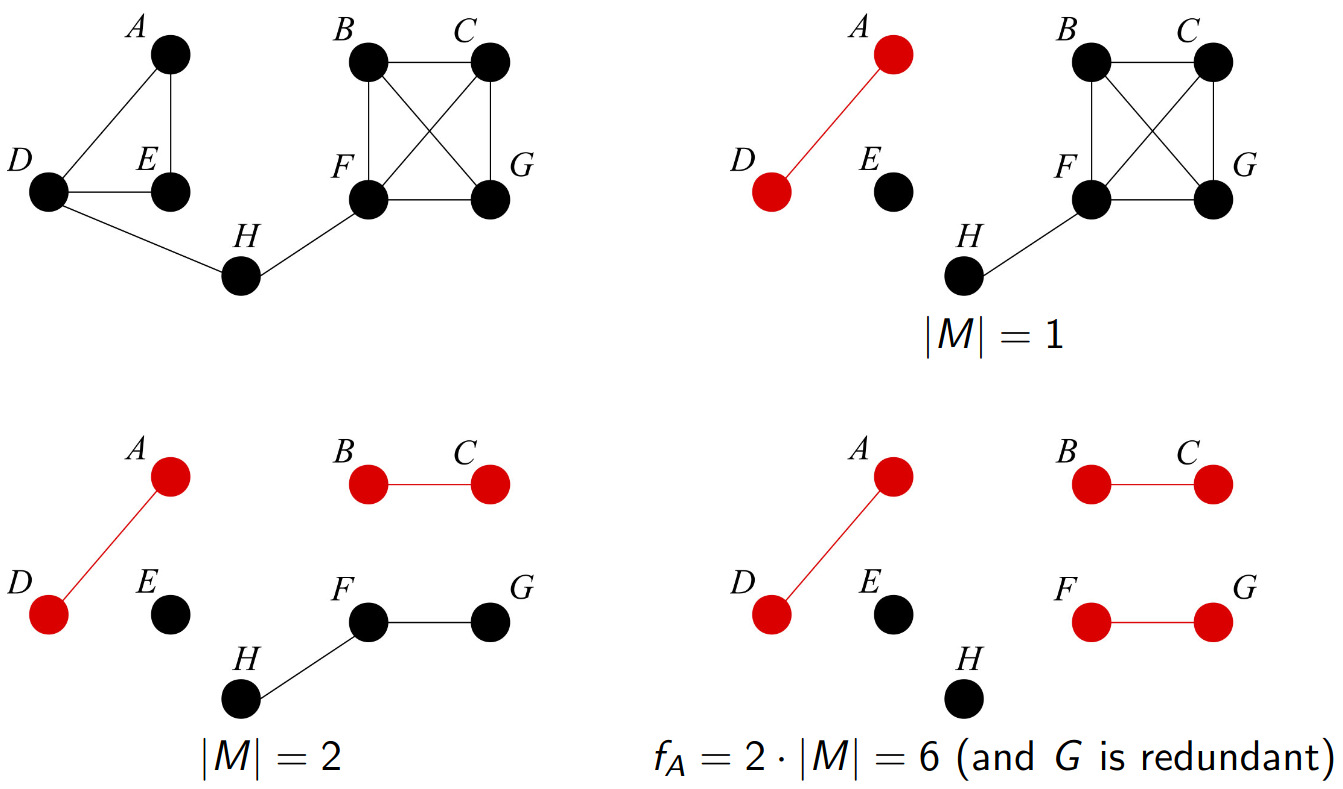
\includegraphics[width=\columnwidth]{img/VCP2Approx}
\end{center}

\textbf{Proof:} The matching algorithm is 2-approximated
\begin{enumerate}
	\item The \textbf{cardinality} of matching $M$ is an \textbf{underestimate} $LB (i )$
	\begin{itemize}
		\item the cardinality of an \textbf{optimal covering} for any subset of edges $E' \subseteq E$ does not exceed that of an optimal covering for $E$
		$$ |x_{E'}^\ast| \leq |x_E^\ast|$$
		(it costs more to cover all edges than only the matching, obviously since the matching is smaller)
		\item the \textbf{optimal covering} of a \textbf{matching} $M$ has \textbf{cardinality} $|M|$ (each edge of the matching requires exactly one different vertex, we're essentially considering half the vertices in the matching, which can cover all the relative edges)
	\end{itemize}
	\item \textbf{Including both} the \textbf{extremes} of each edge of the matching yields
	\begin{itemize}
		\item an \textbf{overestimate} (it covers both the matching and all adjacent edges, i.e. a VCP solution for every maximal matching)
		\item of \textbf{value} $UB (i ) = 2LB (i )$ (two different vertices for each edge, double the cardinality which is our possible $LB (i)$)
	\end{itemize}
	\item The \textbf{matching algorithm} returns \textbf{solutions} of value $f_A (i ) \leq UB (i )$ (possibly removing redundant vertices)
\end{enumerate}
This \textbf{implies} $f_A (i ) \leq 2f^\ast (i )$ for each $i \in I$, since $\alpha_A = 2$.\\

\textbf{And the bound is tight:} Since $\alpha_A$ \textbf{relates} $UB (i )$ and $LB (i )$, $f_A (i )$ and $f^\ast (i )$ could be closer.\\
Actually, for many instances $\rho_A (i )$ is much better than $\alpha_A$.\\

Are there instances $\overline{i}$ for which $f_A (\overline{i}) = \alpha_A f^\ast (\overline{i})$? How are they like? \\
Our value $f_A(i)$ is \textbf{at most} $\alpha_A$ times the \textbf{optimum}, are there instances where our \textbf{solution} is  exactly $\alpha_A$ times the optimal?\\

The study of these instances is useful to
\begin{itemize}
	\item \textbf{evaluate} whether they are \textbf{rare or frequent}
	\item introduce \textbf{ad hoc modifications} to improve the algorithm
\end{itemize}
\begin{center}
	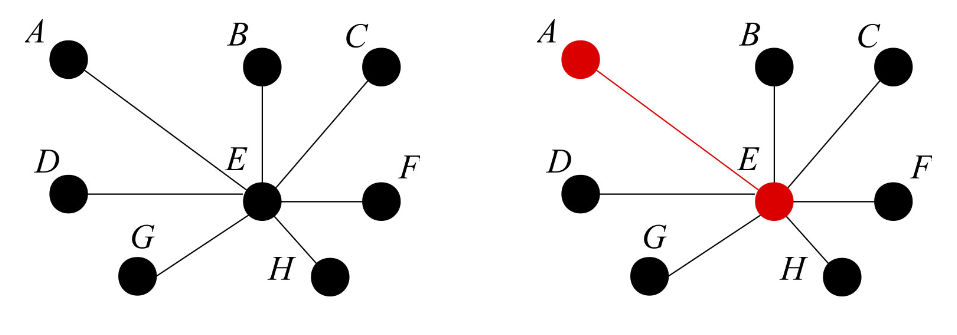
\includegraphics[width=0.8\columnwidth]{img/VCP2Approx2}
\end{center}
In this case our heuristic solution is exactly $\alpha_A$ (2) times the optimum, this is the worst case.\\

In the literature the typical expression "and the bound is tight" introduces the description of instances exhibiting the worst case.\\
If all worst cases are patched, the approximation guarantee improves.\\

\newpage

\paragraph{The TSP under the triangle inequality:} Consider the \textbf{TSP} with the additional (rather common) \textbf{assumptions} that
\begin{itemize}
	\item graph $G = (N, A)$ is \textbf{complete}
	\item cost $c$ is \textbf{nonnegative}, \textbf{symmetric} and \textbf{satisfies} the \textbf{triangle inequality}
	$$ c_{ij} = c_{ji} \;\; \forall i,j \in N \;\; \text{ and } \;\; c_{ij} + c_{jk} \leq c_{ik} \;\; \forall i,j,k \in N $$
	i.e. the road works equally both ways and there can't be roads that connect $i$ and $j$ and subsequently $k$ shorter than the road $ik$ (the costs can form a triangle)
\end{itemize}

\textbf{Double-tree} algorithm
\begin{enumerate}
	\item Consider the \textbf{complete undirected graph} corresponding to $G$
	\item Build a \textbf{minimum cost spanning tree} $T^\ast = (N, X^\ast)$
	\item Make a \textbf{pre-order visit} of $T^\ast$ and build two lists of arcs:
	\begin{enumerate}[label=\alph*.]
		\item $x'$ lists the arcs used \textbf{both} by the \textbf{visit} and the \textbf{backtracking}: this is a circuit visiting each node, possibly several times; exactly twice the cost of the original minimum spanning tree, it's visiting all the nodes
		\item $x$ lists the arcs linking the \textbf{nodes in pre-order ending with the first}: this is a circuit visiting each node exactly once; we use the triangle inequality to go directly across nodes, removing some backtracking and visiting each node only once
	\end{enumerate}
\end{enumerate}

Example:
\begin{center}
	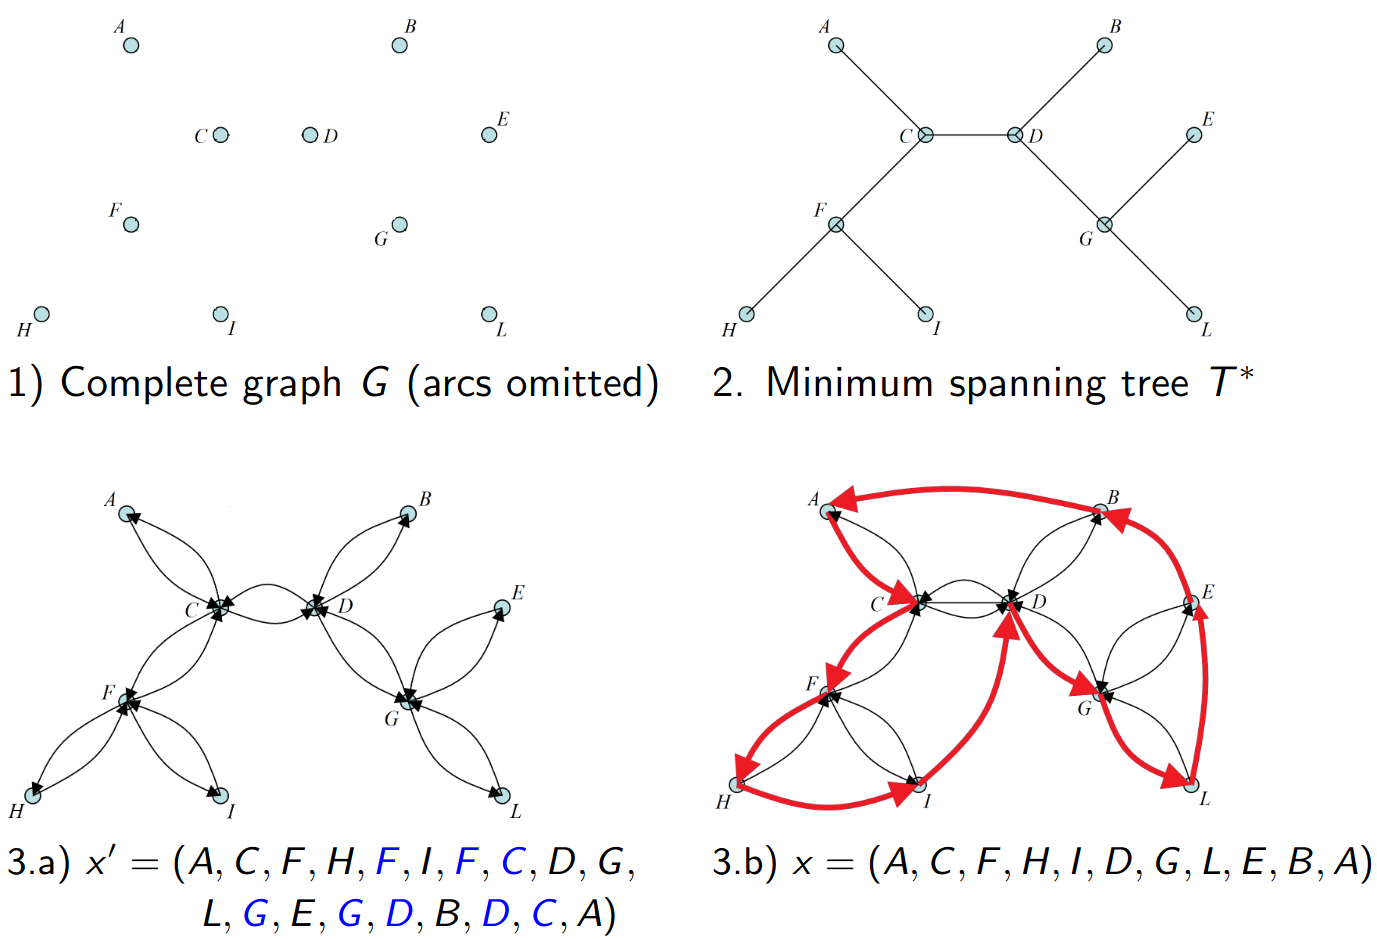
\includegraphics[width=0.8\columnwidth]{img/TSTTI1}
\end{center}

\newpage

The cost of the hamiltonian circuit will be at most equal to twice the spanning tree, which is at most equal to the optimal hamiltonian circuit. The \textbf{cost} is at most \textbf{twice the optimum}. \\

To do the last step you can just look at the path and skip already seen nodes, since it's a complete graph there will be a path to the next unseen node and, as stated by the triangle inequality, it will certainly be $\leq$ than before. \\

This way the result is exactly an hamiltonian circuit, with a cost smaller than the double tree, which has a cost equal to twice the tree, which itself has a cost that smaller than the optimum.\\

The double-tree algorithm is \textbf{2-approximated}:
\begin{enumerate}
	\item the \textbf{cost} of the \textbf{minimum spanning tree} is an \textbf{underestimate} $LB (i )$
	\begin{itemize}
		\item \textbf{deleting} an \textbf{arc} from a Hamiltonian circuit yields a Hamiltonian \textbf{path} that is \textbf{cheaper}
		\item a \textbf{Hamiltonian path} is a \textbf{spanning tree} (usually not of minimum cost)
	\end{itemize}
	\item the \textbf{cost} of circuit $x'$ is
	\begin{itemize}
		\item an \textbf{overestimate} $UB (i )$ (it is a non-minimum Hamiltonian circuit)
		\item \textbf{equal} to $2LB (i )$ (two arcs correspond to each edge)
	\end{itemize}
	\item the \textbf{cost} of circuit $x$ is $f_A (i ) \leq UB (i )$ (a single direct arc replacing a sequence decreases the cost)
\end{enumerate}
This \textbf{implies} that $f_A (i ) \leq 2f^\ast (i )$ for each $i \in I$, so we get $\alpha_A = 2$.\\

Notice: $x'$ is used in the approximation proof, but doesn't need to be computed.\\

\newpage

\paragraph{Inapproximability:} For an inapproximable problem, \textbf{approximated algorithms would be exact}.\\
Consider this family of TSP instances on \textbf{complete graphs} $G = (N, A_0)$:
\begin{itemize}
	\item $c_{ij} = 0$ for $(i, j) \in A_0$
	\item $c_{ij} = 1$ for $(i, j) \in  (N \times N) \setminus A_0$ (the \textbf{triangle inequality is violated}, the earlier approximation can't be applied anymore)
\end{itemize}
Essentially, some arcs are $0$, some $1$, triangle inequality cannot hold.\\

The \textbf{optimum} of any such instance $\overline{i}$ is:
\begin{displaymath}
	\begin{cases}
		f^\ast (\overline{i}) = 0 & \text{ if } A_0 \text{ contains a hamiltonian circuit} \\
		f^\ast (\overline{i}) \geq 1 & \text{ otherwise}
	\end{cases}
\end{displaymath}
(in the latter case, the optimal solution contains at least an arc $\notin A_0$, i.e. an arc that costs $1$).\\

Assume that a \textbf{polynomial algorithm} $A$ provides a \textbf{guarantee} $\alpha_A$
$$ f^\ast (i) \leq f_A (i) \leq \alpha f^\ast (i) \;\; \forall i \in I $$
Then $f^\ast (\overline{i}) = 0 \Leftrightarrow f_A (\overline{i}) = 0$.\\

Whenever the subgraph $G = (N, A_0)$ has a Hamiltonian circuit, our algorithm $A$ necessarily finds it, solving an $\np$-complete problem in polynomial time (and thus $\mathcal{P} = \np$, unlikely as this is of the millennium problems).\\

\newpage

\paragraph{Approximation schemes:} For hard problems
\begin{itemize}
	\item \textbf{exact} algorithms provide the \textbf{best} approximation \textbf{guarantee} ($\alpha_A = 1$, they are exact after all), but require \textbf{exponential time} $T_A$
	\item \textbf{approximated} algorithms provide a \textbf{worse guarantee} ($\alpha_A > 1$), but could require \textbf{polynomial time} $T_A$
\end{itemize}

Some problems admit a \textbf{family of algorithms} providing a whole \textbf{range of compromises} between \textbf{efficiency} ed \textbf{effectiveness}
\begin{itemize}
	\item better and better approximation guarantees: $\alpha_{A_1} > \, ... \, > \alpha_{A_r}$
	\item worse and worse computational complexities: $T_{A_1} < \, ... \, < T_{A_r}$
\end{itemize}
We can have multiple algorithms with different guarantees.\\

Approximation scheme is a parametric algorithm $A_\alpha$ allowing to choose $\alpha$ (Example: the KP).\\

\newpage

\subsubsection{Beyond the worst case}
As usual, the worst-case approach is rough: some algorithms often have a good performance, though sometimes bad.\\

The \textbf{alternative approaches} are similar to the ones used for complexity
\begin{itemize}
	\item \textbf{parametrisation:} prove an \textbf{approximation guarantee} that \textbf{depends} on \textbf{other parameters} of the instances besides the size $n$
	\item \textbf{average-case:} assume a \textbf{probability distribution} on the \textbf{instances} and evaluate the \textbf{expected value} of the approximation factor; the probability affects only the approximation factor, which is reasonable to assume can vary among instances (the algorithm could have a bad performance only on rare instances)
\end{itemize}

but there is at least \textbf{another approach}: 
\begin{itemize}
	\item \textbf{randomization:} the \textbf{operations} of the algorithm \textbf{depend} not only on the instance, but \textbf{also on pseudo-random numbers}, so that the \textbf{solution} becomes a \textbf{random variable} which can be investigated (the time complexity could also be random, but usually is not).\\ 
	Random numbers are used to make decisions inside the algorithm, running it several time provides different results, the distribution of such results can be studied, usually in relation to the random seed used for each specific iteration. \\
\end{itemize}

\newpage

\subsubsection{Randomized approximation algorithms}
For a randomised algorithm $A$, $f_A (i , \omega)$ and $\rho_A (i , \omega)$ are random variables depending on the pseudo-random number seed $\omega$.\\

A randomised approximation algorithm has an approximation ratio whose expected value is limited by a constant
$$ E \left[\rho_A (i, \omega)\right] \leq \alpha_A \text{ for each } i \in I $$

\paragraph{Randomized approximation for the MAX-SAT:} given a CNF, find a truth assignment to the logical variables that satisfy a maximum weight subset of formulae.\\

Purely \textbf{random algorithm:} Assign to each variable $xj$ $(j = 1, \, ... \, , n)$
\begin{itemize}
	\item value \textit{False} with probability $1/2$
	\item value \textit{True} with probability $1/2$
\end{itemize}
What is the \textbf{expected value} of the solution? \\

Let $\delta_i (x)$ be 1 if solution $x$ satisfies clause $i$, 0 otherwise.\\

The \textbf{objective} $f (x) = f_A (I , \omega)$ is the \textbf{total weight} of the \textbf{satisfied clauses} and its expected value is
$$ E \left[f_A (i, \omega)\right] = E \left[\sum_{i \in C} \delta_i (x) w_i \right] = \sum_{i \in C} \left(w_i \cdot Pr \left[\delta_i (x) = 1\right]\right)$$
The total sum is equal to the weight of the satisfied clauses ($C$ contains all clauses, when not satisfied they are multiplied by $\delta_i (x) \implies 0$), this depends on the random seed, so the expected value is the weight of each clause multiplied by the probability of having a satisfied clause.\\

\newpage

Our \textbf{probability} is a number between zero and one and we need to \textbf{estimate it}.\\
Let $k_i$ be the number of literals of formula $i \in C$ and $k_{min} = \min_{i \in C} k_i$ (minimum number of literals among all the clauses)
$$ Pr \left[\delta_i (x) = 1\right] = 1 - \left(\frac{1}{2}\right)^{k_i} \geq 1 - \left(\frac{1}{2}\right)^{k_{min}} \text{ for each } i \in C $$
$$ \implies E \left[f_A (i, \omega)\right] \geq \sum_{i \in C} w_i \cdot \left[1 - \left(\frac{1}{2}\right)^{k_{min}}\right] = \left[1 - \left(\frac{1}{2}\right)^{k_{min}}\right] \sum_{i \in C} w_i $$
The first line essentially represents the probability of each clause not having a single "good" literal, which will at least be $1 - (1/2)^{k_{min}}$ since $k_{min}$ is the minimum number of literals $\implies$ highest probability of not satisfying the clause.\\
The second row is a minorization of the probability of each clause (kinda like an underestimate of the probability).\\

And since $\sum_{i \in C} w_i \geq f^\ast (i)$ for each $i \in I$ \textbf{one obtains}
$$ \frac{E \left[f_A (i, \omega)\right]}{f^\ast (i)} \geq \left[1 - \left(\frac{1}{2}\right)^{k_{min}}\right] \geq \frac{1}{2} $$

This is an incredibly simple algorithm, but the sample average of many iterations will tend to get near the theoretical the expected value, but the best of the many iterations will certainly better than the average and consequently better than the theoretical approximation.\\

% End of L4

\newpage

\subsection{Empirical analysis}
The theoretical analysis is \textbf{complicated} by the fact that
\begin{itemize}
	\item the steps of the algorithm have a \textbf{complex effect} on the \textbf{solution} though usually \textbf{not} on the \textbf{computational cost}
	\item \textbf{average} case and \textbf{randomization} require a \textbf{statistical treatment}
\end{itemize}
The theoretical analysis can be \textbf{unsatisfactory} in practice when its conclusions are based on \textbf{unrepresentative assumptions}
\begin{itemize}
	\item an \textbf{infrequent worst case} (very hard and very rare instances)
	\item an \textbf{unrealistic} probability \textbf{distribution} of the instances
\end{itemize}

\textbf{Experimental analysis} chooses a \textbf{benchmark} of instances and \textbf{measures performance} on that specific set (obviously not all possible instances).\\

The experimental approach is very common in science
\begin{itemize}
	\item mathematics is an exception, based on the formal approach
	\item algorithmics is an exception within the exception, you can get useful information from practical performances
\end{itemize}
The basics of the \textbf{experimental approach} are
\begin{enumerate}
	\item start from \textbf{observation}
	\item formulate a \textbf{model} (work hypothesis)
	\item repeat the following steps
	\begin{enumerate}[label=\alph*.]
		\item \textbf{design} computational \textbf{experiments} to validate the model
		\item \textbf{perform} the experiments and collect their results
		\item \textbf{analyze} the \textbf{results} with quantitative methods
		\item \textbf{revise} the \textbf{model} based on the results
	\end{enumerate}
	until a \textbf{satisfactory model} is obtained
\end{enumerate}

\newpage

What is a "\textbf{model}" in the study of algorithms? 
\begin{itemize}
	\item in physics the laws that rule the behavior of phenomena, an assumption about the physical law that affects a certain phenomenon
	\item in \textbf{algorithmics} the \textbf{laws} that \textbf{rule the behavior} of algorithms, assumptions on the laws that an algorithm follows
\end{itemize}

The \textbf{experimental analysis} of algorithms \textbf{aims} to
\begin{itemize}
	\item obtain \textbf{compact indices of efficiency} and \textbf{effectiveness} of an algorithm
	\item \textbf{compare} the \textbf{indices} of different algorithms to rank them
	\item \textbf{describe} the \textbf{relation} between the performance \textbf{indices and parametric values} of the instances (size $n$, etc...)
	\item \textbf{suggest improvements} to the algorithms
\end{itemize}
I can assume that my algorithm will be linear/quadratic/ecc in respect of the size/any other parameter, these are assumptions based on the knowledge of the algorithm and even experiments. This can give a descriptive model regarding the behavior of the algorithm, leading to some technological modifications to improve the algorithm itself.\\

\newpage

\subsubsection{Benchmark sample}
As not all instances can be tested, a benchmark sample must be defined.\\

A meaningful \textbf{sample} must \textbf{represent different}
\begin{itemize}
	\item \textbf{sizes}, in particular for the analysis of the computational cost; size largely determines the complexity and possibly the quality of the solution
	\item \textbf{structural features} (in the case of graphs: density, degree, diameter, ...; any type of index regarding a specific structure)
	\item \textbf{types}
	\begin{itemize}
		\item of \textbf{application}: logistics, telecommunications, production, ...
		\item of \textbf{generation}: realistic, artificial, transformations of other problems
		\item of \textbf{probabilistic} distribution: uniform, normal, exponential, ...
	\end{itemize}
	instances can come from different sources, affecting efficiency
\end{itemize}

Looking for an "\textbf{equiprobable}" benchmark sample \textbf{is meaningless} because the instance sets are infinite and infinite sets do not admit equiprobability (big statistic question).\\

On the contrary, we can \textbf{define} finite \textbf{classes of instances} that are
\begin{itemize}
	\item \textbf{sufficiently hard} to be instructive
	\item \textbf{sufficiently frequent} in applications to be of interest
	\item \textbf{quick enough} to solve to provide sufficient data for inferences
\end{itemize}
and \textbf{extract benchmark samples} from these classes.

\newpage

\paragraph{Reproducibility:} The scientific method requires \textbf{reproducible and controllable results}
\begin{itemize}
	\item concerning the \textbf{instances}, one must use
	\begin{itemize}
		\item publicly available instances
		\item new instances made available to the community
	\end{itemize}
	\item concerning the \textbf{algorithm}, one must specify
	\begin{itemize}
		\item all implementation details
		\item the programming language
		\item the compiler
	\end{itemize}
	\item concerning the \textbf{environment}, one must specify
	\begin{itemize}
		\item the machine used
		\item the operating system
		\item the available memory
		\item ... 
	\end{itemize}
\end{itemize}
Every detail about the instance must be specified to get the same results, even seemingly negligible details can matter in some instances (e.g. different compilers should provide the same result but may yield somewhat different performances).\\

Reproducing results obtained by others is always extremely difficult, these are guidelines but there are limitations (reproducing the machine for example).\\

\newpage

\subsubsection{Comparing heuristic algorithms}
A heuristic algorithm is \textbf{better} than another one when it \textbf{simultaneously}
\begin{itemize}
	\item obtains \textbf{better results}
	\item requires a \textbf{smaller time}
\end{itemize}
Slow algorithms with good results and fast algorithms with bad results \textbf{cannot be compared in a meaningful way} (what if the second had yielded better results if given more time?).\\

It can be justified to \textbf{neglect the computational} time when
\begin{itemize}
	\item considering a \textbf{single algorithm} with no \textbf{comparison} 
	\item comparing algorithms that perform the \textbf{same operations} (e.g., variants of the same algorithm obtained modifying a numerical parameter)
	\item comparing algorithms that mostly perform the same operations with \textbf{few different} ones that take a \textbf{negligible fraction of the time} (e.g., different initializations or perturbations)
\end{itemize}

\paragraph{A statistical model of algorithm performance:} the idea is modeling the execution of algorithm $A$ as if it was a random experiment
\begin{itemize}
	\item the whole set of \textbf{instances} $I$ is the sample space
	\item the benchmark \textbf{subset} of instances $\overline{I} \subset I$ is the \textbf{sample}
	\item the \textbf{computational time} $T_A (i)$ is a random variable; the time required by algorithm $A$ on instance $i$
	\item the \textbf{relative difference} $\delta_A (i )$ is a random variable; the difference of the result obtained by $A$ on $i$ with the optimal result, divided by the optimal result
\end{itemize}
and the statistical properties of the random variables $T_A (i )$ and $\delta_A (i )$ describe the \textbf{performance} of $A$. Both $T_A (i)$ and $\delta_A (i)$ are random variables because they depend on the instance. \\

Instead of considering all the possible values of the computational time and relative difference, we are describing the random variables $T_A (i)$ and $\delta_A (i)$, with their statistical properties, their description will give a description of the performances of the algorithm.\\

\newpage

\paragraph{Estimates of $\delta_A (i)$:} The computation of $\delta_A (i)$ requires to know the optimum $f^\ast (i)$:
$$ \delta_A (i) = \frac{|f_A (i) - f^\ast (i)|}{f^\ast (i)}$$
What if the \textbf{optimum} is \textbf{unknown}? If we can't have an exact optimum value, we need to get an estimate (form below or above, depending on if it's a minimization or maximization problem).\\
Replace it with an underestimate $LB (i )$ and/or an overestimate $UB (i )$
$$ LB (i ) \leq f^\ast (i) \leq UB (i ) \implies \frac{1}{LB(i)} \geq \frac{1}{f^\ast (i)} \geq \frac{1}{UB(i)} \implies $$
$$ \implies \frac{f_A(i)}{LB(i)} - 1 \geq \frac{f_A(i)}{f^\ast (i)} - 1 \geq \frac{f_A(i)}{UB(i)} - 1 $$
$$ \frac{f_A(i)}{f^\ast (i)} - 1 = \begin{cases}
	\delta_A (i) \text{ (minimization) } & \implies \frac{f_A(i) - UB(i)}{UB(i)} \leq \delta_A (i) \leq \frac{f_A(i) - LB(i)}{LB(i)} \\
	- \delta_A (i) \text{ (maximization) } & \implies \frac{UB(i) - f_A(i)}{UB(i)} \leq \delta_A (i) \leq \frac{LB(i) - f_A(i)}{LB(i)}
\end{cases}$$
and therefore
$$ \frac{|f_A(i) - UB(i)|}{UB(i)} \leq \delta_A (i) \leq \frac{|f_A(i) - LB(i)|}{LB(i)} $$
This range yields a region estimate for the SQD diagram.\\

\newpage 

\subsubsection{Analysis of the computational time}
\paragraph{The Run Time Distribution (RTD) diagram:} the RTD is the plot of the \textbf{distribution function} of $T_A (i )$ on $\overline{I}$ (time required on an instance $i$ on the given benchmark)
$$ F_{T_A} (t) = Pr \left[T_A (i) \leq t \right] \text{ for each } t \in \mathbb{R} $$
It gives the \textbf{probability} that the \textbf{execution time} is below a time $t$. \\

Since $T_A (i )$ strongly depends on the size $n (i )$, meaningful RTD diagrams usually refer to \textbf{benchmarks} $\overline{I}_n$ with \textbf{fixed} $n$ (and possibly other fixed parameters suggested by the worst-case analysis).
\begin{center}
	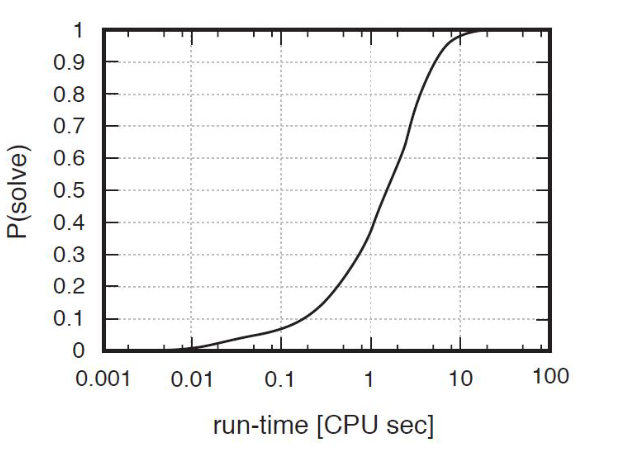
\includegraphics[width=0.75\columnwidth]{img/RTD1}
\end{center}
If given only $n$ as a parameter there are really slow and really fast instances, there could be another parameter which plays a role in the execution time. Essentially dividing $\overline{I}_n$ in further "sub-classes".\\

If all influential parameters are identified and fixed, the RTD diagram degenerates into a step function (all instances require the same time; zero probability under a value, 1 over).\\

\newpage

The Run Time Distribution (RTD) diagram is
\begin{itemize}
	\item \textbf{monotone nondecreasing:} more instances are solved in longer times
	\item \textbf{step-wise and right-continuous:} the graph steps up at each $T (i )$
	\item \textbf{equal to zero for $t < 0$:} no instance is solved in negative time
	\item \textbf{equal to} $1$ \textbf{for} $t \geq \max_{i \in \overline{I}} T(i)$: all are solved within the longest time
\end{itemize}
\begin{center}
	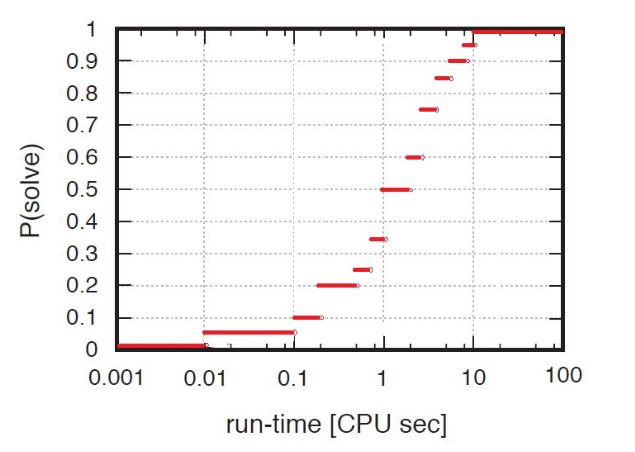
\includegraphics[width=0.75\columnwidth]{img/RTD2}
\end{center}
For large benchmark samples, the plot looks continuous, but it is not.\\

The graph goes up by steps because it shows how many instances (in percent) are solved given a certain amount of time. \\
If there is a big enough number of instances the number of "steps" will increase, giving the impression of a continuous graph.\\

In order to \textbf{build the diagram}:
\begin{enumerate}
	\item \textbf{run} the algorithm \textbf{on each instance} $i \in \overline{I}$
	\item \textbf{build the set} $T_A (\overline{I}) = \left\{T_A (i): \, i \in \overline{I}\right\}$ (it's just a set of numbers)
	\item \textbf{sort} $T_A (\overline{I})$ by \textbf{non-decreasing} values: $t_1 \leq \, ... \, \leq  t_{|\overline{I}|}$
	\item \textbf{plot the points} $\left(t_j, \frac{j}{|\overline{I}|}\right)$ for $j = 1, \, ... \, , |\overline{I}|$ (for each $t_j$ , only the highest) and the horizontal segments (close on the left, open on the right)
\end{enumerate}

\newpage

\paragraph{Scaling diagram:} this diagram describes the dependence of $T (i )$ on the size $n (i )$
\begin{itemize}
	\item \textbf{generate a sequence of values} of $n$ and a sample $\overline{I}_n$ for each value (generate a benchmark sample for each size)
	\item \textbf{apply the algorithm} to each $I \in \overline{I}_n$ for all $n$ (all instances of each sub-benchmark for all the sizes)
	\item \textbf{sketch} all points $(n (i ) , T (i ))$ or the mean points $\left(n, \frac{\sum_{i \in \overline{I}_n} T(i)}{|\overline{I}_n|}\right)$ 
	\item assume an \textbf{interpolating function}
	\item \textbf{estimate the numerical parameters} of the interpolating function
\end{itemize}
It shows how the computational time scales in relation to the size of the instance.
\begin{center}
	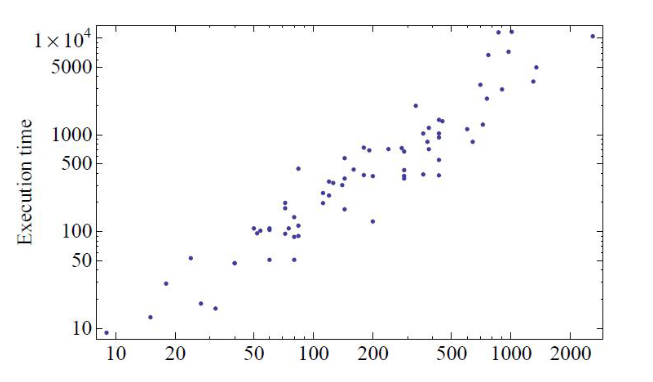
\includegraphics[width=0.7\columnwidth]{img/SD1}
\end{center}
This analysis provides an \textbf{empirical average-case complexity}
\begin{itemize}
	\item with \textbf{well-determined multiplying factors} (instead of $c_1$ and $c_2$)
	\item \textbf{not larger} than the \textbf{worst-case one} (it also includes easy instances)
\end{itemize}

\newpage

The correct family of interpolating functions can be suggested
\begin{itemize}
	\item by a \textbf{theoretical analysis} (studying the algorithm)
	\item by \textbf{graphical manipulations}
\end{itemize}
(Linear interpolation is usually the right tool).\\

The \textbf{scaling diagram turns into a straight line} when
\begin{itemize}
	\item an \textbf{exponential algorithm} is represented on a \textbf{semi-logarithmic scale} (the logarithm is applied only to the time axis)
	$$ \log_2 T(n) = \alpha n + \beta \Leftrightarrow T(n) = 2^\beta \left(2^\alpha\right)^n $$
	if the $\log$ of the time is a linear function of the size, necessarily the algorithm is exponential.\\
	I see the time goes up a lot, I have reason to suspect the algorithm is exponential from the theoretical analysis $\implies$ I try to use a logarithmic scale for the time.\\
	
	\item a \textbf{polynomial algorithm} is represented on a \textbf{logarithmic scale} (the logarithm is applied to both axes)
	$$ \log_2 T(n) = \alpha\log_2 n + \beta \Leftrightarrow T(n) = 2^\beta n^\alpha $$
	the $\log$ of the time is a $\log$ function of the size, then the computational time is polynomial ($\alpha$ is the exponent).\\
\end{itemize}

\newpage

\subsubsection{Analysis of the quality of the solution}
The \textbf{Solution Quality Distribution (SQD) diagram} is the plot of the \textbf{distribution function} of $\delta_A (i)$ \textbf{on} $\overline{I}$ (relative difference on the benchmark)
$$ F_{\delta_A} (\alpha) = Pr \left[\delta_A (i) \leq \alpha\right] \text{ for each } \alpha \in \mathbb{R} $$
\begin{center}
	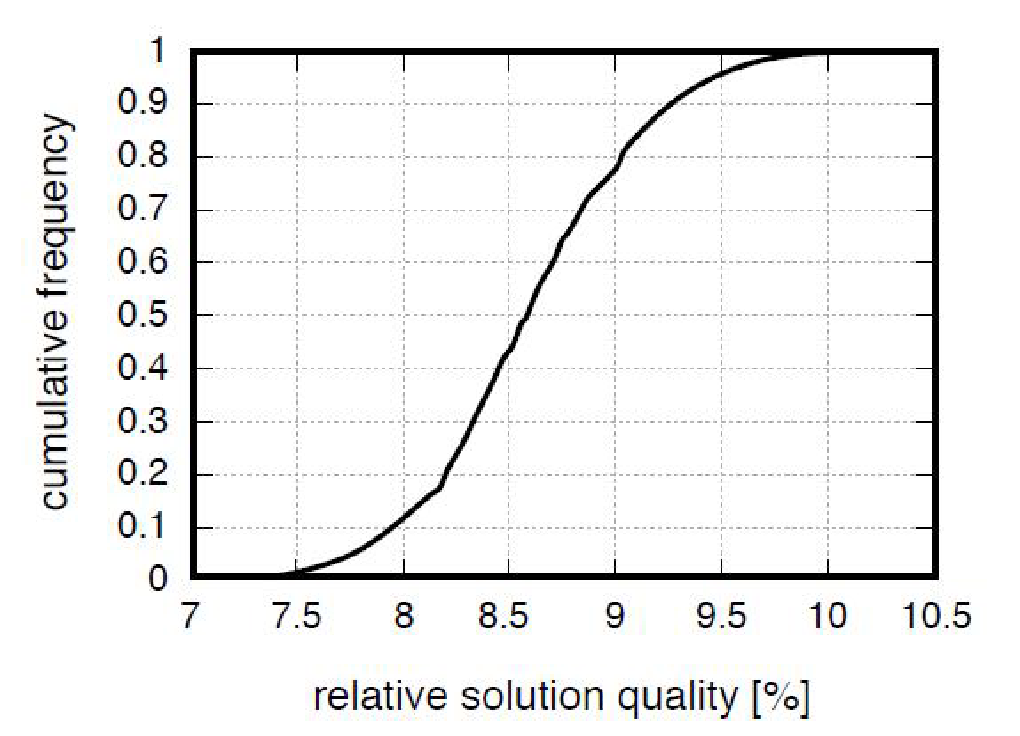
\includegraphics[width=0.7\columnwidth]{img/SQD1}
\end{center}
It plots the probability that the relative difference is smaller than a value $\alpha$, for each possible value of $\alpha$. \\

One axis is the frequency, the other is the relative difference, it basically answers the question "how many instances got this $\delta_A$ or less?". \\

\newpage

For any algorithm, the \textbf{distribution function} of $\delta_A (i)$ is
\begin{itemize}
	\item \textbf{monotone non-decreasing:} more instances are solved with worse gaps
	\item \textbf{step-wise and right-continuous:} the graph steps up at each $\delta (i)$
	\item \textbf{equal to zero for $\alpha < 0$:} no instance is solved with negative gap
	\item \textbf{equal to $1$ for $\alpha \geq \max_{i \in \overline{I}} \delta (i)$:} all are solved within the largest gap
\end{itemize}
\begin{center}
	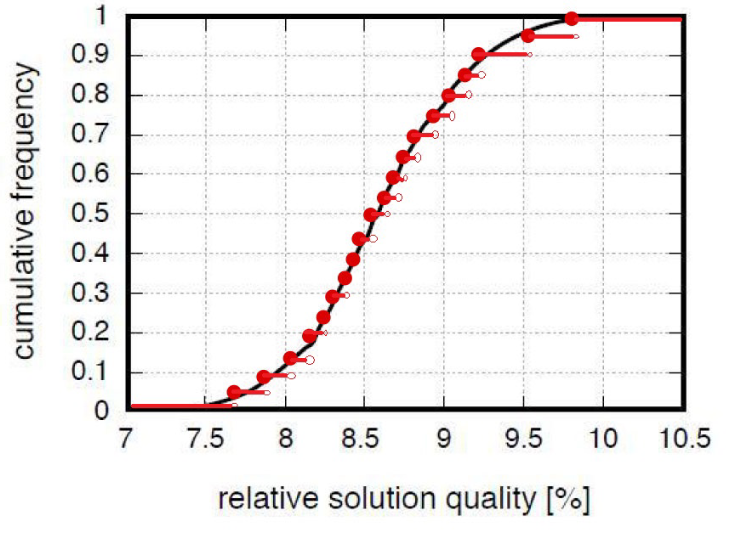
\includegraphics[width=0.7\columnwidth]{img/SQD2}
\end{center}
As with the RTD, the more instances you have the more this diagram looks continuous.\\

If $A$ is an
\begin{itemize}
	\item exact algorithm, it is a step-wise function, equal to $1$ for all $\alpha \geq 0$
	\item $\overline{\alpha}$-approximated algorithm, it is a function equal to $1$ for large $\alpha$
\end{itemize}
\nn

In order to \textbf{build the diagram}:
\begin{enumerate}
	\item \textbf{run the algorithm on each instance} $i \in \overline{I}$
	\item \textbf{build the set} $\Delta_A (\overline{I}) = \left\{\delta_A (i): \, i \in \overline{I} \right\}$, the relative difference for each instance (you need the optimum, could be approximated)
	\item \textbf{sort} $\Delta_A (\overline{I})$ non-decreasing values: $\delta_1 \leq \, ... \, \leq \delta_{|\overline{I}|}$
	\item \textbf{plot points} $\left(\delta_j, \frac{j}{|\overline{I}|}\right)$ for $j = 1, \, ... \, , |\overline{I}|$ (for each $\delta_j$, only the highest) and the horizontal segments (close on the left, open on the right)
\end{enumerate}

\newpage

\paragraph{Parametric SQD diagrams:} Given the theoretical and practical problems to build a \textbf{meaningful sample} often the \textbf{diagram is parameterized} with respect to
\begin{itemize}
	\item a \textbf{descriptive parameter of the instances} (size, density, ...)
	\item a \textbf{parameter} of the \textbf{probability distribution assumed} for the \textbf{instances} (expected value or variance of the costs, ...)
\end{itemize}
\begin{center}
	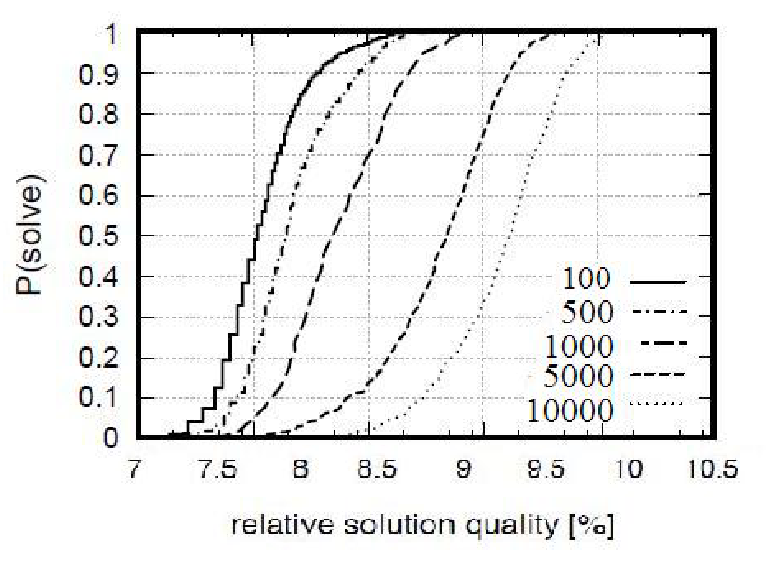
\includegraphics[width=0.7\columnwidth]{img/SQD3}
\end{center}
The conclusions are more limited, but the \textbf{sample is more significant}. General trends can be highlighted (what happens as size increases?).\\

It's basically dividing the benchmark set into sub-benchmarks, following some parameters (such as size, ecc...), to get the solution quality in relation to those parameters. \\

\newpage

\paragraph{Comparison between algorithms with the SQDs:} How to determine whether an \textbf{algorithm is better than another}? (for simplicity's sake, the algorithms take the same time)
\begin{itemize}
	\item \textbf{strict dominance:} it obtains better results on all instances
	$$ \delta_{A_2} (i) \leq \delta_{A_1} (i) \text{ for each } i \in I $$
	This usually happens only in trivial cases (e.g., $A_2$ "includes" $A_1$). $A_2$ is always better. \\
	
	\item \textbf{probabilistic dominance:} the distribution function has higher values for every value of $\alpha$
	$$ F_{\delta_{A_2}} (\alpha) \geq F_{\delta_{A_1}} (\alpha) \text{ for all } \alpha \in \mathbb{R} $$
	the SQD of $A_2$ is larger or equal than the one for $A_1$ (is "above", if you set a certain threshold of "quality" $A_2$ has a better occurrence rate).\\
\end{itemize}

The following plot shows no dominance, but $A_1$ is less "robust" than $A_2$: $A_1$ has results more dispersed than $A_2$ (both better and worse)
\begin{center}
	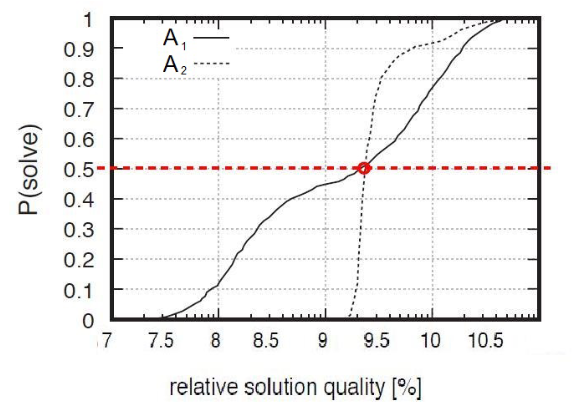
\includegraphics[width=0.7\columnwidth]{img/SQD4}
\end{center}

% End of L5

\newpage

\subsubsection{Compact statistical descriptions}
The distribution function $F_{\delta_A}$ can be replaced or accompanied by more compact characterizations of the effectiveness of an algorithm.\\

This typically involves classical \textbf{statistical indices} of 
\begin{itemize}
	\item \textbf{position}, such as the sample mean
	$$ \overline{\delta}_A = \frac{\sum_{i \in \overline{I}} \delta_A (i)}{|\overline{I}|} $$
	\item \textbf{dispersion}, such as the sample variance
	$$ \overline{\sigma}_A^2 = \frac{\sum_{i \in \overline{I}} \left(\delta_A (i) - \overline{\delta}_A \right)^2}{|\overline{I}|} $$
\end{itemize}
These indices "\textbf{suffer}" from the influence of \textbf{outliers}.\\

Other statistical indices are "stabler" and more detailed
\begin{itemize}
	\item the \textbf{sample median}
	\item suitable \textbf{sample quantiles}
\end{itemize}

\newpage

\subsubsection{Boxplots diagrams}
\paragraph{Boxplot:} A graphic representation is the boxplot (or box and whiskers diagram)
\begin{itemize}
	\item sample \textbf{median} ($q_{0.5}$)
	\item \textbf{lower} and \textbf{upper} sample \textbf{quartiles} ($q_{0.25}$ and $q_{0.75}$)
	\item the \textbf{extreme} sample values (often excluding the "outliers")
\end{itemize}
\begin{center}
	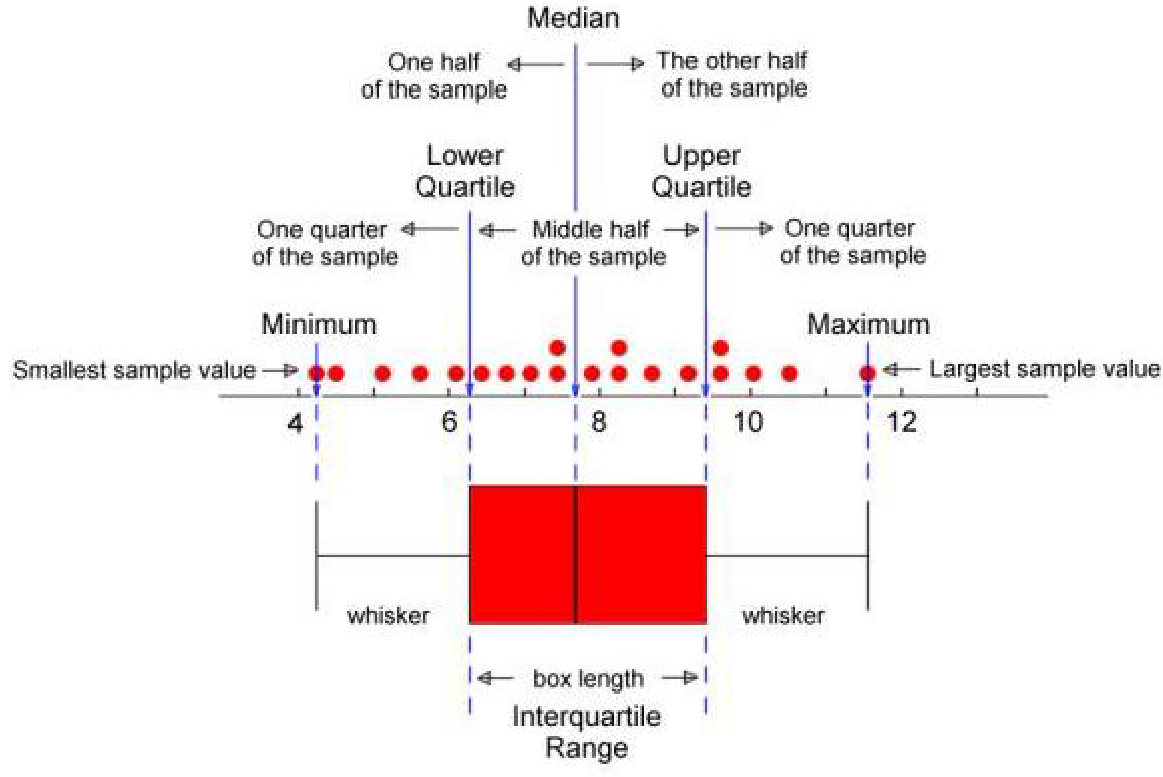
\includegraphics[width=0.9\columnwidth]{img/boxplot1}
\end{center}
On the $x$ axis there's the relative difference (in the example, from $4$ to $12$). The median is in the middle, the box represents the two middle quartiles, the whiskers represent the last two quartiles.\\

To have a boxplot diagram you need to have: extreme values (upper and lower), lower and upper quartiles, median. If you have these values you can draw the diagram.\\

\newpage

\paragraph{Comparison between algorithms with boxplot diagrams:} A more compact comparison can be performed with boxplot diagrams (the dots represent outliers)
\begin{center}
	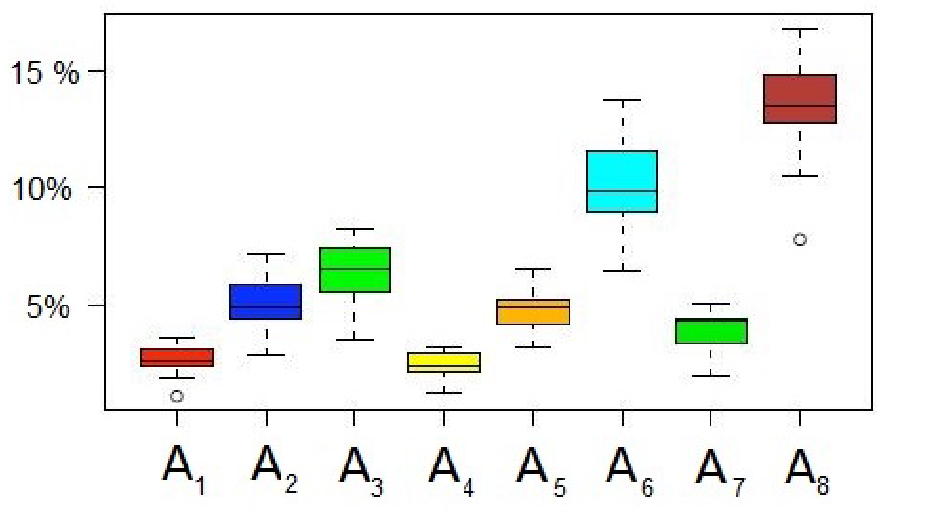
\includegraphics[width=0.9\columnwidth]{img/boxplot2}
\end{center}
\textbf{Necessary} conditions:
\begin{center}
	\textbf{Strict dominance} $\implies$ \textbf{Probabilistic dominance} $\implies q_i \leq q_i ' (i = 1, \, ... \, , 5)$
\end{center}
Strict dominance holds only if probabilistic dominance holds. \\

\textbf{Strict dominance} holds if a boxplot is \textbf{fully below the other} (e.g. $A_7 - A_8$).\\

\textbf{Probabilistic dominance} holds only if \textbf{each} of the five \textbf{quartiles} is \textbf{not above} the corresponding \textbf{one of the other} algorithm (e.g. $A_2 - A_3$).\\

Strict dominance means a box is fully below another, probabilistic dominance means a box is at least partially below another. Obviously the first implies the latter.\\

\newpage

\subsubsection{Relation between quality and computational time}
Many heuristic algorithms find \textbf{several solutions} during their execution, instead of a single one, and consequently can be \textbf{terminated prematurely}.\\

In particular, \textbf{metaheuristics} (random steps or memory mechanisms) have a computational time $t$ fixed by the user and potentially unlimited; they often find a solution and improve on it.\\

Let $\delta_A (i, t)$ be the \textbf{relative difference} reached by $A$ at time $t$ on instance $i$.\\
As a function of time $t$, $\delta_A (i, t)$ is
\begin{itemize}
	\item $+ \infty$ if $A$ has \textbf{not} yet \textbf{found} a feasible \textbf{solution} at time $t$
	\item step-wise \textbf{monotone nonincreasing} (the solution doesn't get worse)
	\item \textbf{constant} after the regular \textbf{termination} ($t \geq T (i)$; after the termination of the algorithm the solution doesn't improve)
\end{itemize}

\vfill

\paragraph{Randomized algorithms:} For randomized algorithms the relative difference $\delta_A (i, \omega, t)$ depends on
\begin{enumerate}
	\item the \textbf{instance} $i \in I$
	\item the \textbf{outcome} $\omega \in \Omega$ of the random experiment guiding the algorithm (the random seed)
	\item the \textbf{execution time} $t$
\end{enumerate}

Given a \textbf{fixed time}, these algorithms can be \textbf{tested}
\begin{enumerate}
	\item on a \textbf{sample of instances} $\overline{I}$ with a \textbf{fixed seed} $\omega$
	\item on a \textbf{fixed instance} $i$ with a \textbf{batch of seeds} $\overline{\Omega}$ (different runs)
	\item on \textbf{several instances} with \textbf{several seeds} on each instance
\end{enumerate}

The results of \textbf{multiple runs} ($\overline{\Omega}$) are usually \textbf{summarized} providing both:
\begin{itemize}
	\item the \textbf{minimum relative difference} $\delta_A^\ast (i, t)$ and the \textbf{total time} $|\overline{\Omega}|t$
	\item the \textbf{average relative difference} $\overline{\delta}_A (i, t)$ and the \textbf{single-run time} $t$
\end{itemize}

\newpage

\subsection{Classification}
The relation between solution quality and computational time allows to \textbf{classify the algorithms} into:
\begin{itemize}
	\item \textbf{complete:} for each instance $i \in I$, find the optimum in finite time
	$$ \exists \overline{t}_i \in \mathbb{R}^+ : \, \delta_A (i, t) = 0 \text{ for each } t \geq \overline{t}, \, i \in I $$
	(Another name for exact algorithms) for every instance the algorithm gives the optimum in finite time. \\
	
	\item \textbf{probabilistically approximately complete:} for each instance $i \in I$, find the optimum with probability converging to $1$ as $t \rightarrow + \infty$
	$$ \lim_{t \rightarrow + \infty} Pr \left[\delta_A (i, t) = 0\right] = 1 \text{ for each } i \in I $$
	(Many randomized metaheuristics) for all instances, the probability of getting an exact solution converges to 1, given enough time. \\
	
	\item \textbf{essentially incomplete:} for some instances $i \in I$, find the optimum with probability strictly $< 1$ as $t \rightarrow + \infty$
	$$ \exists i \in I: \, \lim_{t \rightarrow + \infty} Pr \left[\delta_A (i, t) = 0 \right] < 1 $$
	(Most greedy algorithms, local search algorithms, ...) even given infinite time, some instances can't get to the exact solution. \\
\end{itemize}

\newpage

\subsubsection{Beyond the optimum, a generalization}
An obvious generalization \textbf{replaces} the search for the \textbf{optimum} with that for a \textbf{given level of approximation}
δA (I , t) = 0 → δA (I , t) ≤ α
$$ \delta_A (i, t) = 0 \rightarrow \delta_A (i, t) \leq \alpha $$
We're not searching for an exact solution, we're looking for a "good enough" solution, where the "good enough" is determined by $\alpha$.\\

The algorithms can now be \textbf{classified} in
\begin{itemize}
	\item \textbf{$\alpha$-complete algorithms:} for each instance $i \in I$, find an $\alpha$-approximated solution in finite time ($\alpha$-approximated algorithms).\\
	
	\item \textbf{probabilistically approximately $\alpha$-complete algorithms:} for each instance $i \in I$, find an $\alpha$-approximated solution with probability converging to $1$ as $t \rightarrow + \infty$.\\
	
	\item \textbf{essentially $\alpha$-incomplete algorithms:} for some instances $i \in I$, find an $\alpha$-approximated solution with probability strictly $< 1$ as $t \rightarrow +\infty$
\end{itemize}

In conclusion, every algorithm provides a \textbf{compromise} between
\begin{itemize}
	\item a \textbf{quality measure}, described by the threshold $\alpha$
	\item a \textbf{time measure}, described by the threshold $t$
\end{itemize}

\newpage

\subsubsection{Probability of success}
Let the \textbf{success probability} $\pi_{A, n} (\alpha, t)$ be the probability that algorithm $A$ finds in \textbf{time} $\leq t$ a solution with a \textbf{gap} $\leq \alpha$ on an instance of \textbf{size} $n$
$$ \pi_{A, n} (\alpha, t) = Pr \left[\delta_A (i, t) \leq \alpha | i \in I_n, \, \omega \in \Omega \right]$$
\begin{center}
	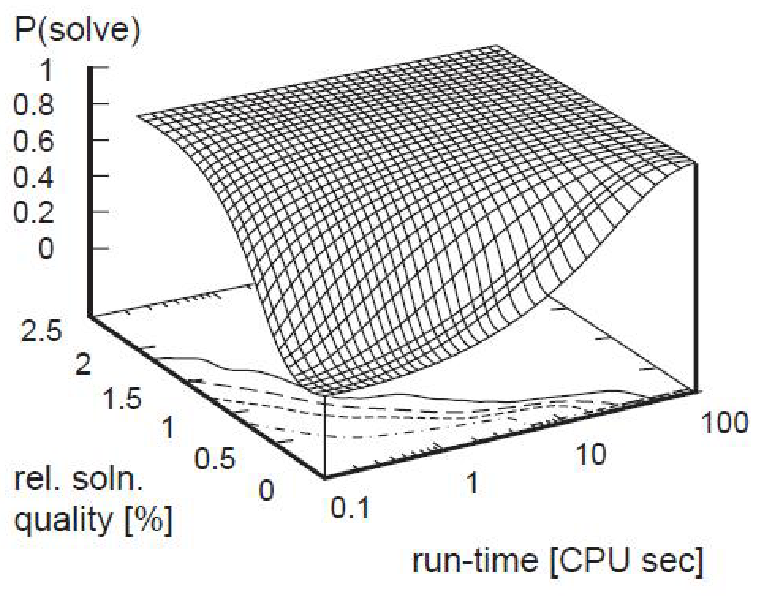
\includegraphics[width=0.7\columnwidth]{img/Psucc1}
\end{center}
This yields different secondary diagrams, derived from the time, solution quality and probability of solving.\\

\newpage

\paragraph{Qualified Run Time Distribution (QRTD) diagrams:} The QRTD diagrams describe the profile of the \textbf{time required} to \textbf{reach} a specified \textbf{level of quality}.
\begin{center}
	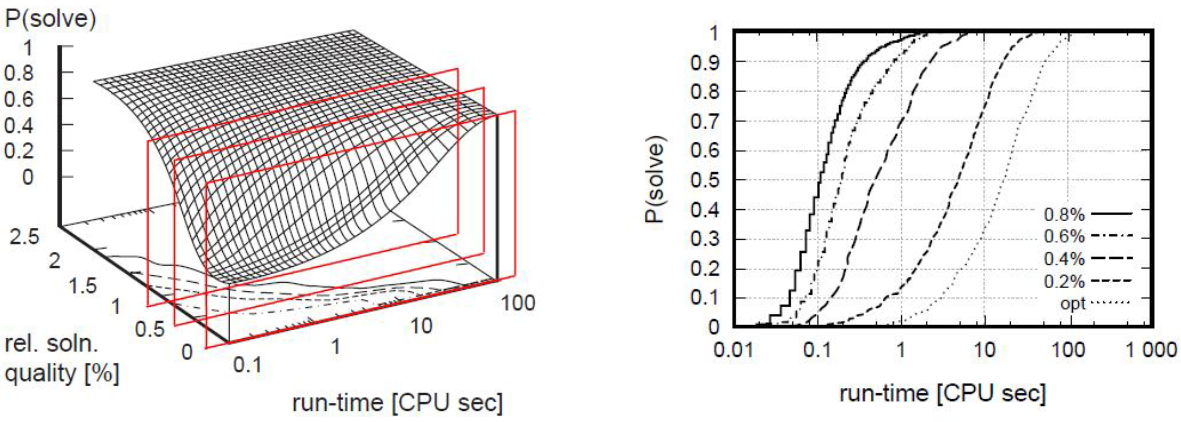
\includegraphics[width=\columnwidth]{img/QRTD1}
\end{center}

This is fixing the quality of the solution $\alpha$ and showing how the probability of getting such quality changes in relation to computational time.\\

They are useful when the computational time is not a tight resource.\\

If the algorithm is
\begin{itemize}
	\item complete, all diagrams reach $1$ in finite time
	\item $\overline{\alpha}$-complete, all diagrams with $\alpha \geq \overline{\alpha}$ reach $1$ in finite time
	\item $\overline{\alpha}$-incomplete, all diagrams with $\alpha \leq \overline{\alpha}$ do not reach $1$
\end{itemize}

\newpage

\paragraph{Timed Solution Quality Distribution (TSQD) diagrams:} The TSQD diagrams describe the profile of the \textbf{level of quality} reached in a \textbf{given computational time}
\begin{center}
	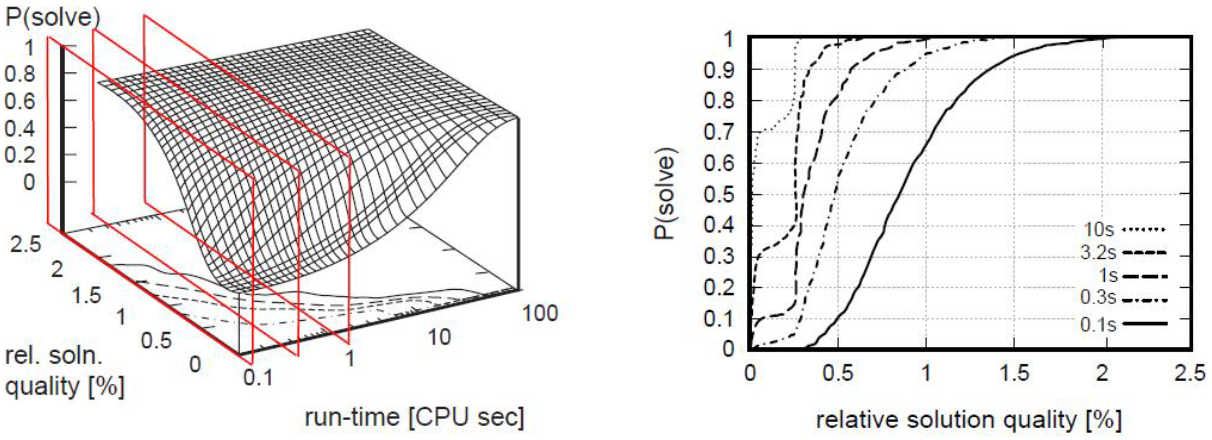
\includegraphics[width=\columnwidth]{img/TSQD1}
\end{center}

This is fixing the computational time and showing what's the probability of getting a certain quality of solution in that given time.\\

They are useful when the computational time is a tight resource.\\

If the algorithm is
\begin{itemize}
	\item complete, all diagrams with a sufficient $t$ are step functions in $\alpha = 0$
	\item $\overline{\alpha}$-complete, all diagrams with a sufficient $t$ reach $1$ in $\alpha = \overline{\alpha}$
	\item probab. approx. $\overline{\alpha}$-complete, the diagrams converge to $1$ in $\alpha = \overline{\alpha}$
	\item $\overline{\alpha}$-incomplete, all diagrams keep $< 1$ in $\alpha = \overline{\alpha}$
\end{itemize}

\newpage

\paragraph{Solution Quality statistics over Time (SQT) diagrams:} One can also draw the \textbf{level lines} associated to \textbf{different quantiles}. 
\begin{center}
	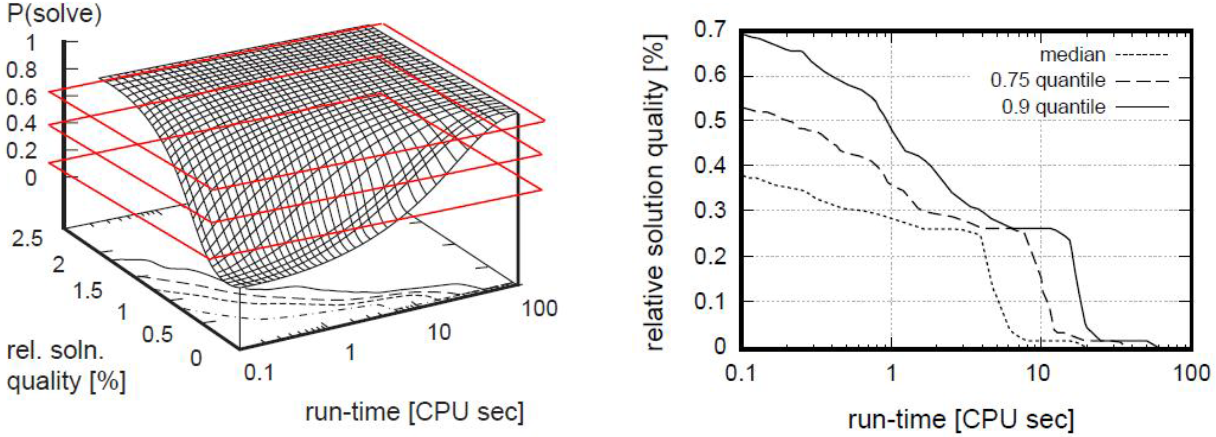
\includegraphics[width=\columnwidth]{img/SQT1}
\end{center}

This shows how the solution quality changes in relation to the computational time, given a fixed probability of getting such quality of solution. \\

They describe the compromise between quality and computational time.\\

For a robust algorithm the level lines are very close to each other.\\

\newpage

\subsection{Statistical tests (Wilcoxon's test)}
Diagrams and boxplots are qualitative: how do you \textbf{evaluate} quantitatively if the \textbf{empirical difference between algorithms} $A_1$ and $A_2$ is \textbf{significant}?\\

\textbf{Wilcoxon's test} focuses on effectiveness (neglecting robustness)
\begin{itemize}
	\item $f_{A_1} (i) - f_{A_2} (i)$ is a \textbf{random variable defined on the sample space} $I$, objective function, measures the quality; if it's negative $A_1$ is better than $A_2$ and vice versa (assuming a minimization problem).\\
	
	\item Formulate a \textbf{null hypothesis} $H_0$ according to which the \textbf{theoretical median} of $f_{A_1} (i) - f_{A_2} (i)$ is \textbf{zero} (they are equivalent, half the time one is better, switching for the other half).\\
	
	\item Extract a \textbf{sample of instances} $\overline{I}$ and \textbf{run} the \textbf{two algorithms} on it, obtaining a \textbf{sample of pairs of values} $(f_{A_1}, f_{A_2})$.\\
	
	\item Compute the \textbf{probability} $p$ of \textbf{obtaining the observed result} (that particular set of pairs) or a more "extreme" one (that set or less probable), assuming that $H_0$ is true (assuming it follows our hypothesis); is it just bad luck or is the hypothesis wrong? \\
	
	\item Set a \textbf{significance level} $\overline{p}$, that is the
	\begin{itemize}
		\item \textbf{maximum acceptable probability to reject} $H_0$ assuming that it is true
		\item that is, to consider \textbf{two identical medians as different}
		\item that is, to consider \textbf{two equivalent algorithms as differently effective} (referring to the median of the gap)
	\end{itemize}
	$\overline{p}$ is the probability above which we can say that the hypothesis follows our observed results.\\
	
	\item \textbf{reject} $H_0$ \textbf{when} $p < \overline{p}$
\end{itemize}
Typical values for the significance level are $\overline{p} = 5\%$ or $\overline{p} = 1\%$.\\

\newpage

\subsubsection{Assumptions} 
It is a \textbf{nonparametric} test, that is, it does \textbf{not} make \textbf{assumptions} on the \textbf{probability distribution} of the tested \textbf{values}.\\

It is useful to evaluate the performance of heuristic algorithms, because the \textbf{distribution of the result} $f_A (i )$ is \textbf{unknown}. \\

It is based on the following \textbf{assumptions}:
\begin{itemize}
	\item \textbf{all data} are \textbf{measured} at least on an \textbf{ordinal scale} (the specific values do not matter, only their relative size, you just need a sequence of levels, we use numbers so it's obviously verified)
	\item the two \textbf{data sets} are \textbf{matched} and \textbf{derive from the same population} (we apply $A_1$ and $A_2$ to the same instances, extracted from $I$, so it's always verified)
	\item each \textbf{pair of values is extracted independently} from the others (the instances are generated independently from one another, not always satisfied)
\end{itemize}

\newpage

\subsubsection{Application}
Application of the Wilcoxon's test: 
\begin{enumerate}
	\item Compute the \textbf{absolute differences} $| f_{A_1} (i_j) − f_{A_2} (i_j)|$ for all $i_j \in \overline{I}$ (instance by instance).\\
	
	\item \textbf{Sort} them by \textbf{increasing} values and assign a \textbf{rank} $R_j$ to each one; all zero-differences can be removed; in case of ties, all should have an average.\\
	We're getting the sum of all the ranks, which is proportional to the difference, this serves the purpose of considering if the difference itself is large or small and not only the number of instances an algorithm has "won".\\
	
	\item Separately \textbf{sum the ranks of the pairs} with a positive difference and those of the pairs with a negative difference
	$$ 
	\begin{cases}
		W^+ & = \sum_{j:f_{A_1} (i_j) > f_{A_2} (i_j)} R_j \\
		W^- & = \sum_{j:f_{A_1} (i_j) < f_{A_2} (i_j)} R_j
	\end{cases}
	$$
	If the null hypothesis $H_0$ were true, the two sums should be equal.\\
	Each positive is summed together, same with the negatives, if the algorithms are truly equivalent (as per the null hypothesis), these should be the same, i.e. $W^+ - W^-$ should be $0$. We're computing the sum of the ranks for the instances where the first algorithm is better than the second and vice versa.\\
	
	\item The \textbf{difference} $W^+ - W^-$ allows to \textbf{compute} the \textbf{value of} $p$: each of the $|\overline{I}|$ differences can be positive or negative: $2^{|\overline{I}|}$ outcomes; $p$ is the fraction with $|W^+ - W^-|$ equal or larger than the observed value.\\
	
	\item if $p < \overline{p}$, the \textbf{difference is significant} and
	\begin{itemize}
		\item if $W^+ < W^-$, $A_1$ is better than $A_2$
		\item if $W^+ > W^-$, $A_1$ is worse than $A_2$
	\end{itemize}
\end{enumerate}

\newpage

\paragraph{Computation of the $p$-value:} The value of $p$ (distribution of probability) is usually
\begin{itemize}
	\item \textbf{computed explicitly} by enumeration when $|\overline{I}| < 20$; which possible cases give us each value?
	\item \textbf{approximated} with a \textbf{normal distribution} when $|\overline{I}| \geq 20$; there's a lot of cases, it can be approximated
\end{itemize}
\begin{center}
	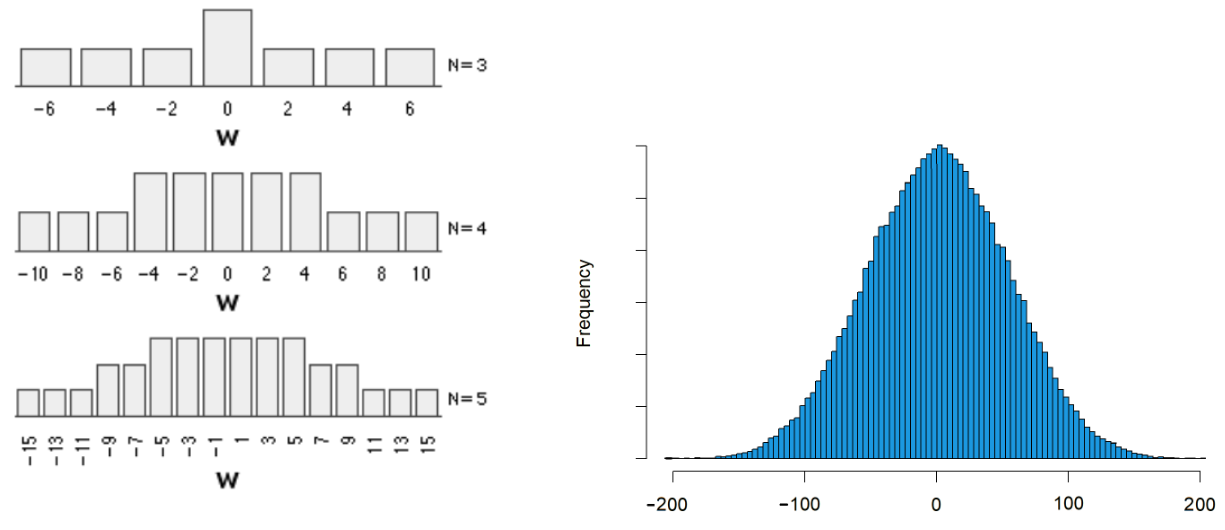
\includegraphics[width=\columnwidth]{img/pval1}
\end{center}
Of course, pre-computed tables also exist.\\

We get the probability distribution and we observe the probability of the value we got, then we need to evaluate if it's reasonable or if it's a significant result. \\

\newpage

\paragraph{Possible conclusions:} Wilcoxon's test can suggest
\begin{itemize}
	\item that \textbf{one of the two algorithms is significantly better} than the other
	\item that the \textbf{two algorithms are statistically equivalent} (but take it as a stochastic response, and keep an eye on $p$)
\end{itemize}

If the sample includes instances of different kinds, two algorithms could be \textbf{overall equivalent}, but \textbf{nonequivalent} on the \textbf{single classes} of instances.\\

\textbf{Dividing the sample} could reveal
\begin{itemize}
	\item classes of instances for which $A_1$ is better
	\item classes of instances for which $A_2$ is better
	\item classes of instances for which the two algorithms are equivalent
\end{itemize}
but multiplying questions means getting some wrong answers by chance (FWER = Family-Wise Error Rate). \\

What about testing $\delta_A (i)$ instead of $f_A (i )$? (Open question).\\

% End of L6

\newpage